\documentclass[12pt,compress,ngerman,utf8,t]{beamer}
\usepackage{etex}
\usepackage[ngerman]{babel}
\usepackage{graphicx}
\usepackage[export]{adjustbox}
\usepackage{multicol}
% \usepackage{animate}
% \usepackage{media9}


\usetheme[numbering=fraction, progressbar=frametitle]{metropolis}


\date{\today}
\institute{University of Freiburg}
\titlegraphic{\vspace{4cm} \hspace{9cm} 
\includegraphics[height=2cm]{template/Logo-Uni-Freiburg.png}}
\graphicspath{ {./template/} {./proseminar/} }

\title{Superturingmaschinen}
\author{Felix Karg}

\newif\ifonline
\onlinefalse
% \onlinefalse

\AtBeginSection[]
{
    \large
    \begin{frame}{Inhalt}
        \begin{multicols}{2}
            \tableofcontents[currentsection]
        \end{multicols}
        \clearpage
    \end{frame}
}

\AtBeginSubsection[]
{
    \large
    \begin{frame}{Inhalt}
        \begin{multicols}{2}
            \tableofcontents[currentsection,currentsubsection]
        \end{multicols}
        \clearpage
    \end{frame}
}

% \vspace{0.1cm}



\newcommand{\code}[1]{
    \begin{center}
    \setlength{\fboxrule}{1pt}
    \setlength{\fboxsep}{8pt}
        {\fbox{\parbox{0.81\textwidth}{#1}}}
   \end{center}
}




\begin{document}

\maketitle

% multicols from:
% https://tex.stackexchange.com/questions/24343/splitting-toc-into-two-columns-on-single-frame-in-beamer

%%%%%%%%%%%%%%%%%%%%%%%%%%%%%%%%%%%%%%%%%%%%%%%%%%%%%%%%%%%%%%%%%%%%%%%%%%%%%%%%%%%%%%%%%%%%%%%%%%%%%%%%%%%%%%%%%%%

\begin{frame}{Inhalt}
    \large
    \begin{multicols}{2}
        \tableofcontents[hidesubsections]
    \end{multicols}
    \clearpage
\end{frame}




%%%%%%%%%%%%%%%%%%%%%%%%%%%%%%%%%%%%%%%%%%%%%%%%%%BEGINNING%%%%%%%%%%%%%%%%%%%%%%%%%%%%%%%%%%%%%%%%%%%%%%%%%%%%%%%%
\section{Recap}



\begin{frame}[c]{}
    \center
    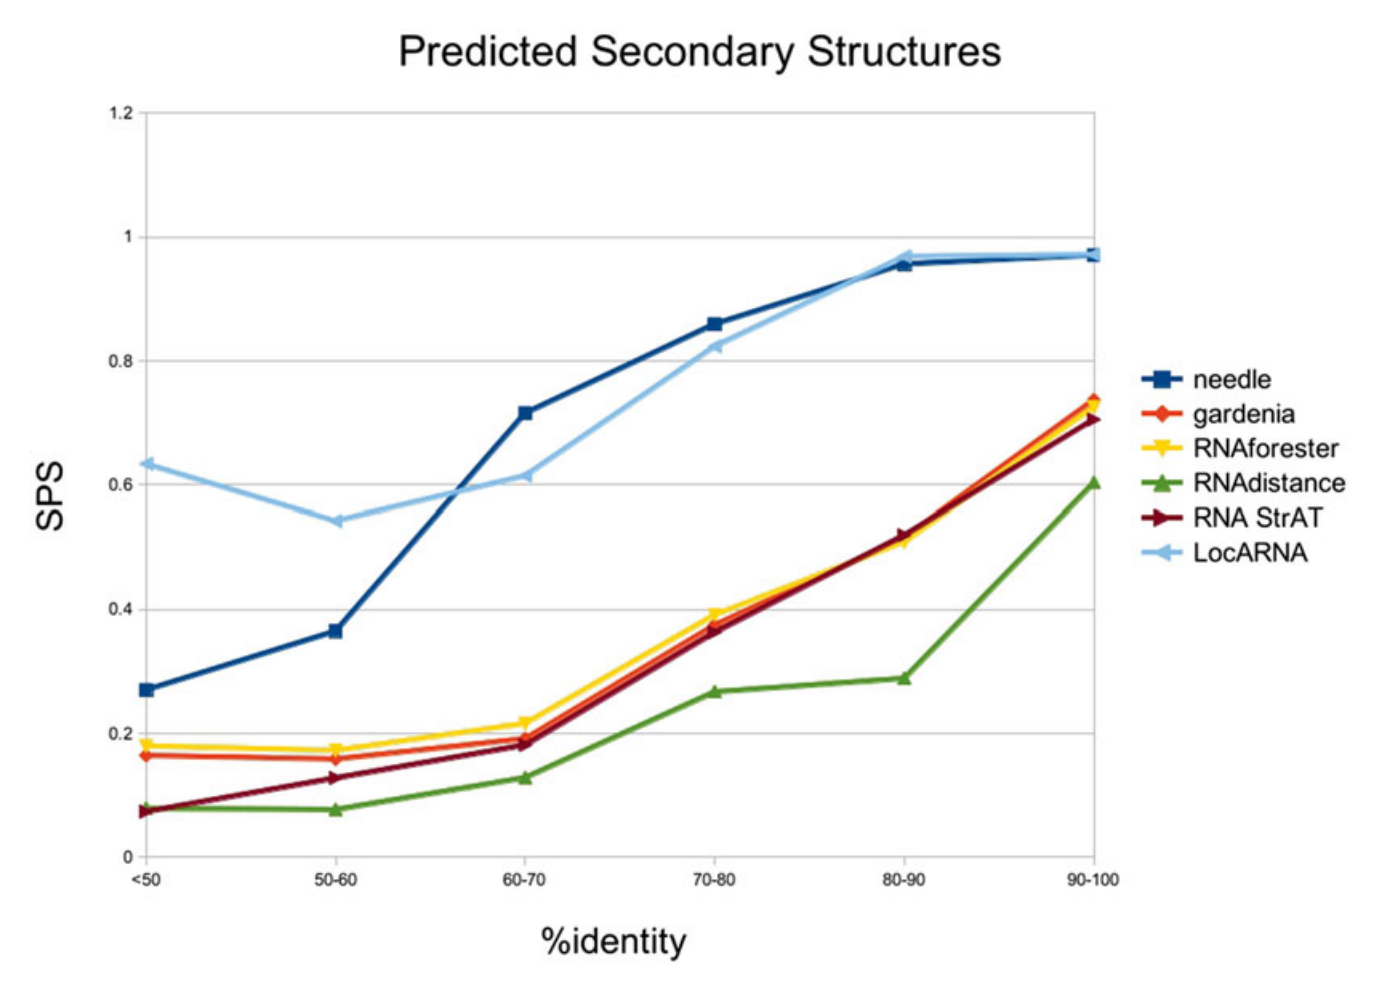
\includegraphics[width=\textwidth]{predicted}
\end{frame}


\begin{frame}[c]{}
    \center
    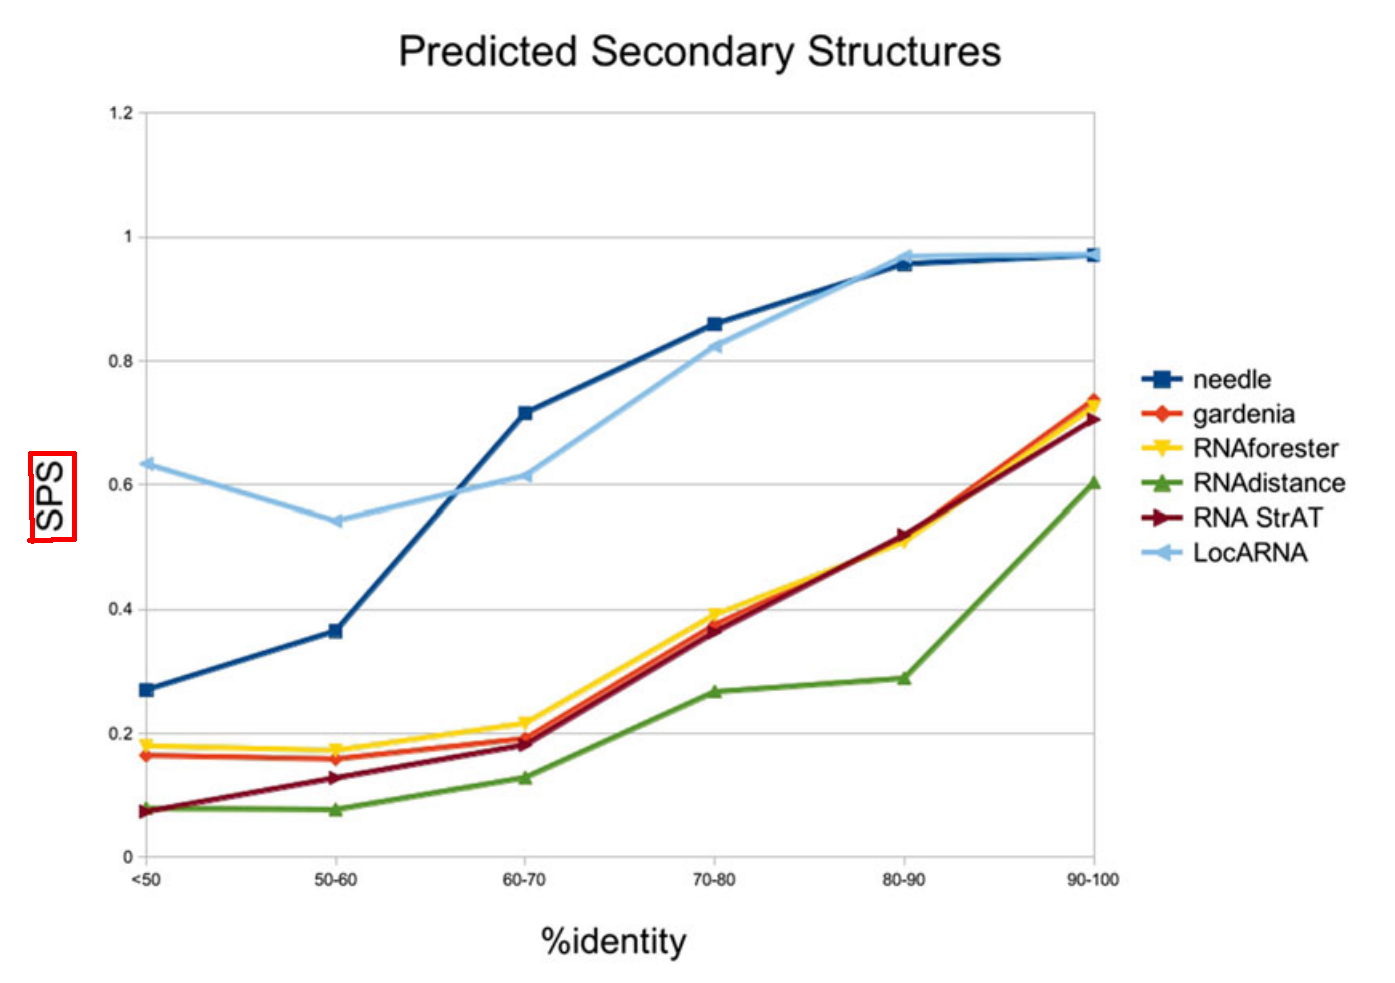
\includegraphics[width=\textwidth]{predicted_sps}
\end{frame}


\begin{frame}[c]{SPS - introduction}
    Sum of Pairs Score
    \newline
%    \vspace{2cm}
    \newline
    \pause
    Used to measure the \only<2-2>{alignment}\only<3->{similiarity} of two RNA sequences
\end{frame}


\begin{frame}[c]{Sequence Similiarity - Example}
    A: \only<4-5>{AAGGC}\only<1-1>{AAGGC}\only<2-3>{{\color{ForestGreen} AAGGC}}\only<1,4->{TT}\only<2-3>{{\color{red}TT}} \\
    B: \only<1-1>{AAGGC}\only<2-5>{{\color{ForestGreen} AAGGC}} \\
    C: \only<1-3>{AAGGC}\only<4->{{\color{ForestGreen} AAGGC}}\only<4-5>{{\color{red}AT}}\only<-3>{AT} \newline
    \newline
    Similiarity: \only<3,5>{60\% = 1 - (2 / 5) } \\
    1 - (edit distance / unaligned length of shorter sequence)
\end{frame}


\begin{frame}[c]{Sequence Similiarity - Example}
    A: {\color{ForestGreen}AAGGC}{\color{red}T}{\color{ForestGreen}T} \\
    B: AAGGC \\
    C: {\color{ForestGreen}AAGGC}{\color{red}A}{\color{ForestGreen}T} \newline
    \newline
    Similiarity: \only<2>{ 86\% = 1 - (1 / 7) } \\
    1 - (edit distance / unaligned length of shorter sequence)
\end{frame}


\begin{frame}[c]{}
    \center
    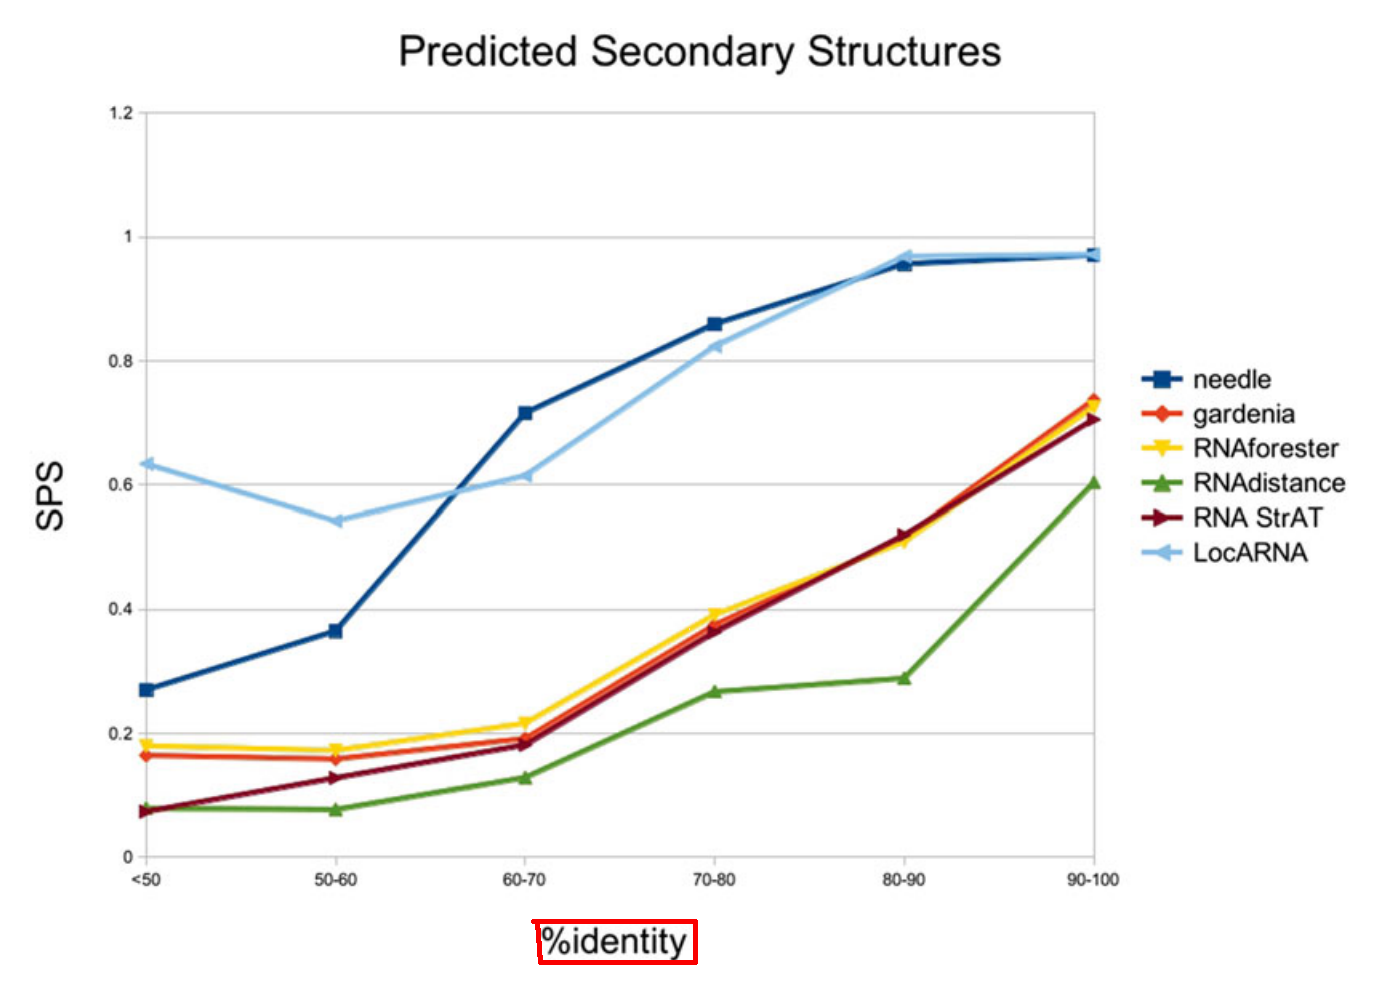
\includegraphics[width=\textwidth]{predicted_identity}
\end{frame}


\begin{frame}[c]{Sequence Identity - Example}
    A: \only<4-5>{AAGGC}\only<1-1>{AAGGC}\only<2-3>{{\color{ForestGreen} AAGGC}}TT \\
    B: \only<1-1>{AAGGC}\only<2-5>{{\color{ForestGreen} AAGGC}} \\
    C: \only<1-3>{AAGGC}\only<4-5>{{\color{ForestGreen} AAGGC}}AT \newline
    \newline
    Identity: \only<3,5>{100\%} \\
    Identical nucleotides / shorter sequence length
\end{frame}


\begin{frame}[c]{Sequence Identity - Example}
    A: {\color{ForestGreen}AAGGC}{\color{red}T}{\color{ForestGreen}T} \\
    B: AAGGC \\
    C: {\color{ForestGreen}AAGGC}{\color{red}A}{\color{ForestGreen}T} \newline
    \newline
    Identity: \only<2>{85\% = 6 / 7} \\
    Identical nucleotides / shorter sequence length
\end{frame}


\begin{frame}[c]{needle}
    \center
    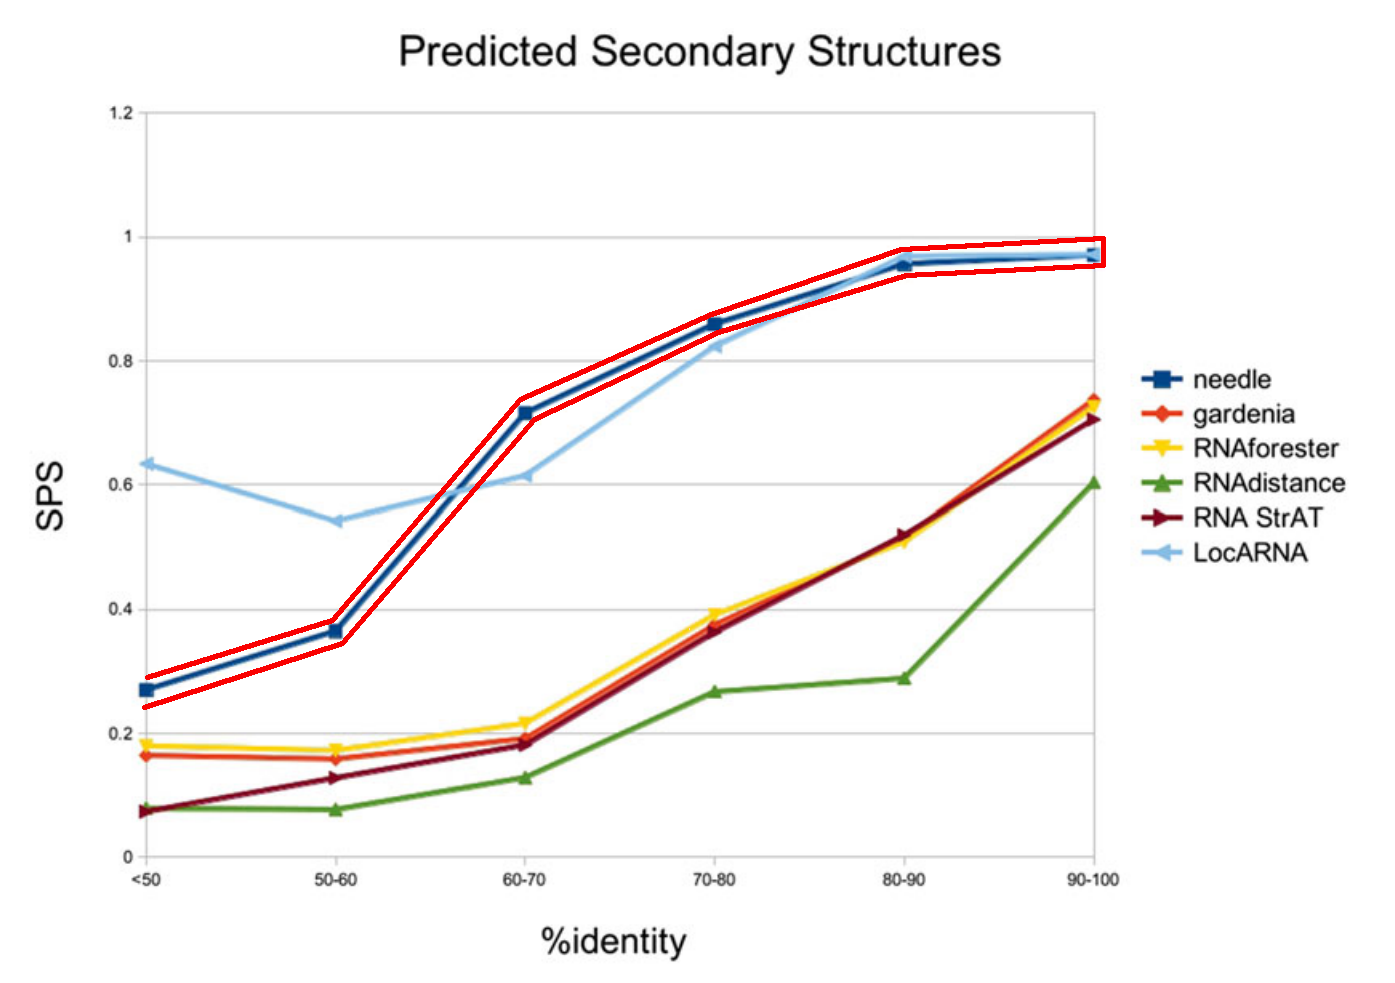
\includegraphics[width=\textwidth]{predicted_needle}
\end{frame}

\begin{frame}[c]{Needleman-Wunsch-Algorithm}
    \center
    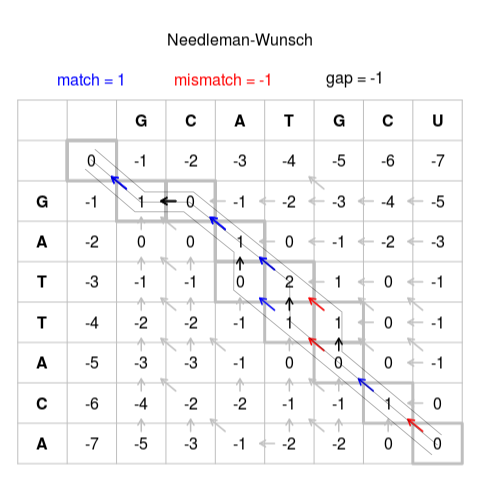
\includegraphics[width=0.75\textwidth]{Needleman-Wunsch_pairwise_sequence_alignment}
\end{frame}











 % PROGRESS
% % \section{Berechenbarkeit}


\begin{frame}[c]{Berechenbarkeit}
    \large
    Verschiedene Modelle:
    \begin{multicols}{2}
        \begin{itemize}
             \item DEA (Deterministischer Endlicher Automat)
             \item PDA (Kellerautomaten)
             \item Turingmaschinen
             \item Superturingmaschine
        \end{itemize}
        \begin{itemize}
            \item Chomsky-Hierarchy Typ 3
            \item Chomsky-Hierarchy Typ 2
            \item Chomsky-Hierarchy Typ 0
            \item kein wirkliches analogon
        \end{itemize}
    \end{multicols}
\end{frame}



\section{Turingmaschinen}

\begin{frame}[c]{Turingmaschine: Einführung}
    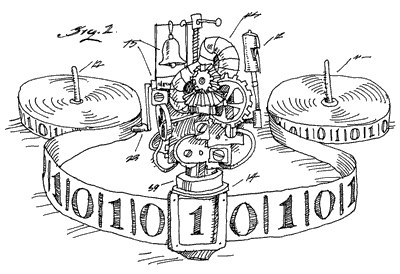
\includegraphics[width=11cm]{turing-machine}
    % Keine Formale Definition, ist bekannt oder eben nicht
    % TM hat:
    % - Unendliches Band mit Zeichen drauf
    % - Lese & Schreibkopf
    % - State-Machine
\end{frame}


\begin{frame}[c]{Turingmaschine: Beispiel}
    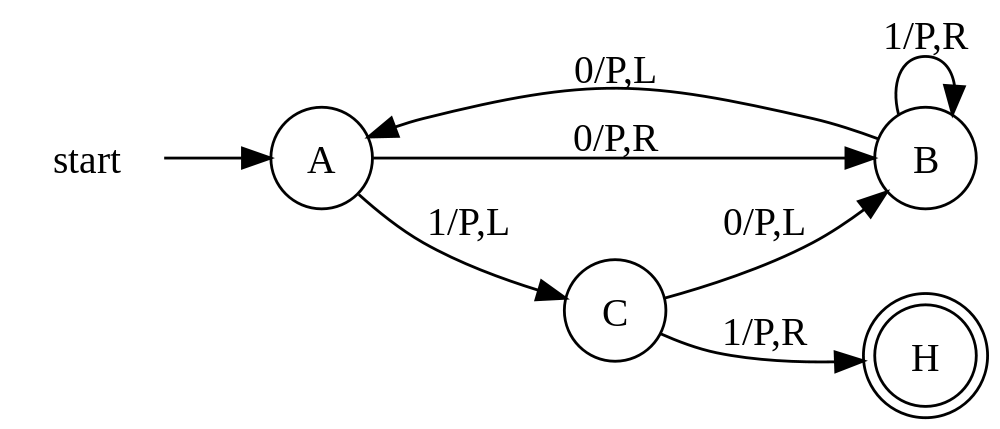
\includegraphics[width=10cm]{tm-ex1} \\
    Schreibt 6 1er auf ein leeres Band.
\end{frame}


\begin{frame}[c]{Eigenschaften von Turingmaschinen}
    Relevant:
    \begin{itemize}
            \pause
        \item Äquivalent zu TM mit mehreren Spuren
            \pause
        \item Äquivalent zu TM mit mehreren Bändern
            \pause
        \item Beliebiges Alphabet (häufig nur Binär)
            \pause
        \item Andere Berechenbarkeitsmodelle gleichmächtig
            \pause
        \item Turingmaschine ist Codierbar
            \pause
        \item Kann andere Turingmaschinen Simulieren
            \pause
        \item Gibt abzählbar unendlich viele
%         \item Halteproblem
    \end{itemize}
\end{frame}



\section{Aussagentypen}



\begin{frame}[c]{Aussagentypen - Einführung}
    \large
    Eine $\Sigma_1$-Aussage ist eine Aussage der Form: \\
    \[ \text{"`Es gibt $n \in \mathbb{N}$ mit $\heartsuit$."',}\]
        \pause
    wobei in der Teilaussage $\heartsuit$ nur noch {\em beschränkte Quantifikatoren} vorkommen dürfen, also Formeln wie:
    \pause
    \[ \text{"`Für alle Zahlen m kleiner .. gilt ..."'} \]
    oder
    \[ \text{"`Es gibt eine Zahl m kleiner .. mit ..."'} \]

\end{frame}


\begin{frame}[c]{Aussagentypen}
    \Large
    $n_1, .., n_k, m_1, .., m_k \in \mathbb{N}$;
    \only<5-> {$f_1, .., f_k : \mathbb{N} \rightarrow \mathbb{N}$} \\
    $M = \{ n \in \mathbb{N}\ |\ \phi(n)\}$ \\

    Aussagen der Form:
    \begin{itemize}
            \pause
        \item $\phi = \exists n_1 .. \exists n_k: \heartsuit$ ( $\Sigma_1$ \only<7> { = NP})
            \pause
        \item $\phi = \exists n_1 .. \exists n_k: \forall m_1 .. \forall m_k: \heartsuit$ ( $\Sigma_2$ )
            \pause
        \item $\phi = \forall n_1 .. \forall n_k: \heartsuit$ ( $\Pi_1$ \only<7> { = co-NP})
            \pause
        \item $\phi = \exists f_1 .. \exists f_k: \heartsuit$ ( $\Sigma_1^1$ )
            \pause
        \item $\phi = \forall f_1 .. \forall f_k: \heartsuit$ ( $\Pi_1^1$ )
    \end{itemize}

\end{frame}




\section{Unendlichkeit}


% \subsection{Kardinalzahlen}
%
% \begin{frame}[c]{Kardinalzahlen}
%     \Large
%     Nur zur Differenzierung
% \end{frame}



% \subsection{Ordinalzahlen}



\begin{frame}[c]{Unendlichkeit allgemein}
    \Large
    Unterschied:
    \pause
    \begin{itemize}
        \item Abzählbar Unendlich \only<4->{($\mathbb{N}, \mathbb{Z}, \mathbb{Q}$)}
            \pause
        \item Überabzählbar Unendlich \only<4->{($\mathbb{R}$)}
    \end{itemize}
\end{frame}



\begin{frame}[c]{Problem des Ordinalen Zahlenstrahls}
    \large
    \only<1> {Normaler Zahlenstrahl: \\}
    \only<2> {Normaler Zahlenstrahl mit ersten Ordinalen Zahlen:\\}
    \Huge
    \only<1> {
        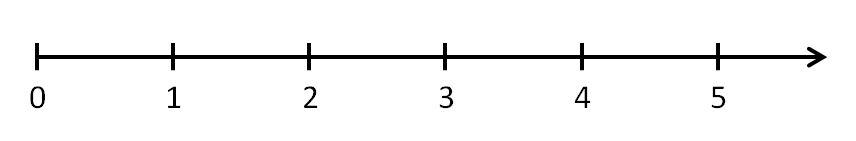
\includegraphics[width=0.8\textwidth]{proseminar/images/zahlenstrahl.jpeg}
        % ganz Normaler Zahlenstrahl, soweit bekannt
        % Zahlen haben Ordinale Eigenschaften
        % Eigenschaften:
        % - Immer entweder Größer, Kleiner oder Gleich
        % - Transitivität
        % - Existenz von Größtem Element in Endlicher Menge
        % Zahlen gehen bis zu unendlich.
        % Frage nach nach dem Ende des Zahlenstrahls
    }

    \only<2> {
        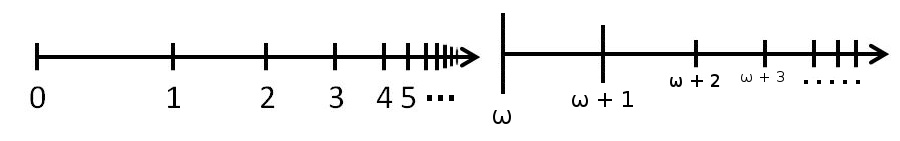
\includegraphics[width=0.85\textwidth]{proseminar/images/zahlenstrahl_ordinal.jpeg}
        % Tadaa! Wir haben zum einen alle 'Normalen' Schritte, haben aber
        % danach immernoch weitere! Wir haben sogar noch Weitere Schritte danach!
    }

    \only<3> {
        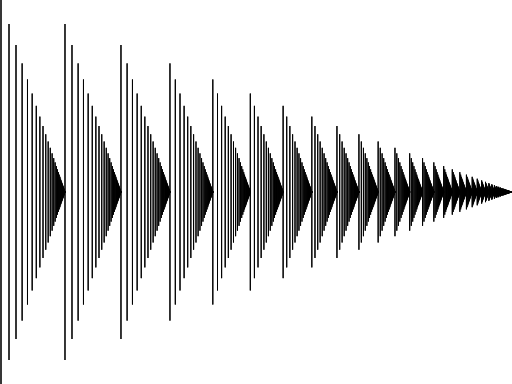
\includegraphics[width=\textwidth]{proseminar/images/ordinal-omega-squared}
        % Das hört da natürlich noch nicht auf, es gibt natürlich noch weitere
        % Stufen, also weitere (explizite) Ordinalzahlen.
        % Bei $\omega * 2$ haben wir also schon 2 mal bis unendlich gezählt!
    }

    \only<4> {
        \hspace{2cm}
        
\includegraphics[height=0.8\textheight]{proseminar/images/ordinal}
        % Es ist so bisschen schwierig das in einen Sinnvollen Zahlenstrahl zu
        % packen ... aber ich hoffe ihr habt verstanden was gemeint ist :)
    }

\end{frame}




% \section{Kardinalzahlen}

\begin{frame}[c]{Kardinalzahlen}
    \Large
    $|\{0, 1, 2\}| = 3$ \pause \\
    $|\{\square, \nabla, \heartsuit\}| = 3$ \\ \pause
    $|\mathbb{N}| = \aleph_0$
\end{frame}


\section{Superturingmaschinen}

\begin{frame}[c]{Superturingmaschinen: Intro}
    \Large
    Eigentlich eine Normale Turingmaschine. \\
    \pause
    Wir Rechnen nur auf einem Ordinalen Zahlenstrahl.
    % Dadurch ergeben sich jetzt erstmal schon so ein paar Fragen,
    % also nach dem Zustand zum Zeitpunkt $\omega$ oder ähnliches.
\end{frame}

\subsection{Grenzverhalten}

\begin{frame}[c]{Grenzverhalten - Unklarheiten}
    \Large
    Was nicht so ganz Klar ist:
    \begin{itemize}
            \pause
        \item In Welchem Zustand sind wir?
            \pause
        \item Wie sieht das Band aus?
            \pause
        \item Was bedeuted das?
    \end{itemize}
\end{frame}


\begin{frame}[c]{Grenzverhalten - Möglichkeiten}
    \Large
    Zwei Möglichkeiten:
    \begin{itemize}
            \pause
        \item Wir halten.
            \pause
            Das ist einfach :)
            \pause
        \item Wir halten nicht.
    \end{itemize}
\end{frame}


\begin{frame}[c]{Grenzverhalten - Erklärung}
    \Large
    \pause
    Es ist echt verdammt schwer GIFs in PDFs zu bekommen ... \\
    \pause
    Demotime. \\
    % Zeige vier Varianten: Immer 1 -> Klar, 1
    % Immer 0 -> Klar, 0
    % Endlich oft 1, unendlich oft 0: immernoch 0
    % Unendlich oft 1, unendlich oft 0: ist 1
    \pause
    { \small
    (Hier werde ich anhand von externen Bildern erklären, wie das Grenzverhalten für Zellen zu verstehen ist)
    }
\end{frame}


\begin{frame}[c]{Grenzverhalten - Beispiel}
    \code{Prüfe im Start- und Limeszustand, ob die aktuelle Zelle eine Eins enthält.
    \begin{itemize}
        \item Wenn Ja, dann halte.
        \item Wenn nein, dann lass die Zelle aufleuchten und laufe ohne Unterlass nach rechts.
    \end{itemize}}
    \pause
    Scheint sich zu wiederholen, hält aber nach Schritt $\omega^2$.

    \bigskip
    \pause
    Eine Superturingmaschine wiederholt sich genau dann, wenn
    \begin{itemize}
        \item die Aufnahmen zu zwei Limesordinalzahlen gleich sind und
        \item zwischen diesen Zeiten keine Zellen, die Null waren zu eins werden.
    \end{itemize}
\end{frame}


\subsection{Fähigkeiten}

\begin{frame}[c]{Fähigkeiten}
    \large
    \begin{itemize}
        \item Alles was Normale Turingmaschinen können
            \pause
        \item Das Klassische Halteproblem lösen
            \pause
        \item Gewisse Zahlentheorethische Aussagen entscheiden
            \pause
        \item Turingmaschinen mit gewissen Fähigkeiten finden
            \pause
        \item Funktionen mit gewissen Eigenschaften finden
            \pause
        \item Die Menge der Wohlordnungen entscheiden
    \end{itemize}
\end{frame}


\begin{frame}[c]{Fähigkeiten II}
    \Large
    Was Superturingmaschinen dennoch nicht können:
    \begin{itemize}
        \item Beliebige 0/1-Folgen auf das Band schreiben
            \pause
        \item Ihr eigenes Halteproblem lösen
            \pause
        \item Beliebig komplexe Aussagen entscheiden
            \pause
        \item Kaffe kochen
            \pause
        \item ...
    \end{itemize}
\end{frame}





% \section{Stempelbare Ordinalzahlen}
\section{Stempelbarkeit}


\begin{frame}[standout]
    \huge
    Können wir zu jeder Natürlichen Zahl halten?
    % Ja, einfach n Zustände.
\end{frame}


\begin{frame}[standout]
    \huge
    Können wir zu jeder Ordinalen Zahl halten?
    % Betrachten wir doch einfach mal an welchen Zahlen wir wirklich halten können.
\end{frame}



% \subsection{Stempelbare Ordinalzahlen - Einführung}
\subsection{Einführung}

\begin{frame}[c]{Stempelbare Ordinalzahlen}
    \pause
    \code{Lese das Band.
    \begin{itemize}
        \item Bei einer 1, halte.
        \item Bei einer 0, schreibe eine 1 und gehe ohne anzuhalten nach rechts.
    \end{itemize}
    }
    \pause
    $\rightarrow$ Wir halten im Schritt $\omega$. \\ \pause
    \small
    (wir haben bereits gesehen dass wir im Schritt $\omega^2$ halten können.)
\end{frame}

\begin{frame}[c]{Erkenntnisse}
    \Large
    \begin{itemize}
        \item Alle Ordinalzahlen bis $\omega^2$ sind Stempelbar.
            \pause
        \item Ist $\alpha$ Stempelbar, so auch $\alpha + \beta$; $\beta \leq \omega^2$.
            \pause
        \item Sind $\alpha$ und $\beta$ Stempelbar, so auch $\alpha + \beta$ \pause und $\alpha * \beta$.
    \end{itemize}
    \pause
    Sind das nicht bereits alle?
\end{frame}


%%%%%%%%%%%%%%%%%%%%%%%%%%%%%%%%%%%%%%%%%%%%%%%%%%%%%%%%%%%%%%%%%%%%%%%%%%%%%%%
\begin{frame}[c]{Speed-Up Lemma}
    \Large
    Wenn $\alpha + n$ Stempelbar ist, so auch $\alpha$.
    % Andersrum klar, aber eigentlich interessant aus einem anderen Grund
    % Kurzfassung: Erkennt Bandinhalt für $\alpha$, setzt gleichzeitig flag.
\end{frame}



\subsection{Lücken-Theoreme}


\begin{frame}[c]{Lücken-Existenz-Theorem}
    \Large
    Es gibt nicht-Stempelbare Lücken in den Ordinalzahlen. Um genau zu sein ist
    die erste Lücke genau $\omega$ groß. \\
    \pause

    Beweis: \pause \\
    Alle Turingmaschinen Simulieren und halten, sobald kein anderes gehalten hat.
\end{frame}


\begin{frame}[c]{Alle Turingmaschinen}
    \Large
    \alt<1,3>{Alle Turingmaschinen}{\underline{\bf Alle Turingmaschinen}} Simulieren und halten, \\
    sobald kein anderes \only<-2>{gehalten}\only<3>{\underline{\bf gehalten}} hat.
    \newline \newline \newline
    Hat es Bedeutung, davon zu sprechen?
    % Zwei dinge die erstmal komisch sind
    % Alle Turingmaschinen -> Annahme: Ja ist möglich, können alle aufschreiben und dementsprechend simulieren
    % gehalten -> starke Annahme: keine Simulierte hält. Ist berechtigt, da es weniger Ordinalzahlen gibt als mögliche TM.
\end{frame}


\begin{frame}[c]{Große-Lücken-Theorem}
    \Large
    Die Lücken werden Groß. Für jede Stempelbare Ordinalzahl gibt es mindestens
    eine genausogroße Lücke.
    \newline
    \newline
    \pause
    Beweis.
    % Zähle durch alle Ordinalzahlen, zähle $\alpha$ am rand mit solange keine
    % hält, wenn alpha durch ist: Lücke gefunden, andernfalls setze \alpha
    % zurück und fange von vorne an. Muss existieren, sonst sind wir irgendwann
    % nach den 'stempelbaren Ordinalzahlen' und können anhalten sobald wir
    % \alpha abgezählt haben.
\end{frame}


\begin{frame}[c]{Viele-Lücken-Theorem}
    \Large
    Es gibt für jede schreibbare Zahl $\alpha$ mindestens $\alpha$ viele
    mindestens $\alpha$ große Lücken in den stempelbaren Ordinalzahlen.
    % Beweis folgt.
\end{frame}


\begin{frame}[c]{Viele-Lücken-Theorem}
    \Large
    Um genau zu sein: ist $\alpha$ Stempelbar oder Schreibbar, ist die Anzahl
    der Lücken mit der Größe mindestens $\alpha$ weder Stempelbar noch
    Schreibbar.
    % Beweis:
    % Wir zählen die Lücken der Größe \alpha und clocken damit \beta.
    % Irgendwann sind wir durch, und damit also hinter den stempelbaren
    % Ordinalzahlen, wenn wir jetzt halten haben wir einen Widerspruch, also
    % kann \beta weder stempelbar noch schreibbar sein.
\end{frame}





\section{Halteprobleme}



\section{Sources}

%%%%%%%%%%%%%%%%%%%%%%%%%%CITES%%%%%%%%%%%%%%%%%%%%%%%%%%%%%
\begin{frame}[c,fragile,allowframebreaks]{Sources}
    The slides can be found at: \newline \newline

    \beamertemplatearticlebibitems
    \begin{thebibliography}{10}

    \bibitem{Github}
        {\bf Github}
        \newblock \url{https://github.com/fkarg/things-to-talk-about/tree/master/bioinfII}
    \newline

    \bibitem{Needleman-Wunsch Image}
            {\bf Needleman-Wunsch Image}
            \newblock \url{https://upload.wikimedia.org/wikipedia/commons/3/3f/Needleman-Wunsch_pairwise_sequence_alignment.png}

    \bibitem{Secondary structures Image}
            {\bf Secondary structures Image}
            \newblock \url{https://www.sciencedirect.com/science/article/pii/B9780124200371000014}

    \bibitem{RNA-Bioinformatics Lecture}
            {\bf RNA-Bioinformatics Lecture}
            \newblock \url{https://ilias.uni-freiburg.de/ilias.php?ref_id=1009368&obj\_id=1&cmd=layout&cmdClass=illmpresentationgui&cmdNode=fu&baseClass=ilLMPresentationGUI}


%     \beamertemplatebookbibitems
%     \bibitem{Richard Rumelt}
%         Richard Rumelt
%         \newblock {\em Good Strategy / Bad Strategy}.
%         \newblock The Difference and Why It Matters \\
%                   ISBN: 978-1-78125-154-6
%     \beamertemplatearticlebibitems
%     \bibitem{Lesswrong}
%         Lesswrong
%             \newblock {\em Expecting short Inferential Distances}
%             \newblock \url{http://lesswrong.com/lw/kg/expecting\_short\_inferential\_distances/}
%     \bibitem{Lesswrong}
%         Lesswrong
%             \newblock {\em Cached Thoughts}
%             \newblock \url{http://lesswrong.com/lw/k5/cached\_thoughts/}
%     \bibitem{Zenhabits}
%         Zenhabits
%             \newblock {\em say No so you can say YES}
%             \newblock \url{https://zenhabits.net/say-yes/}
%
%     \bibitem{Wikiquote}
%         Fukuzawa Yukichi
%             \newblock {\em Wikiquote}
%             \newblock \url{https://en.wikiquote.org/wiki/Fukuzawa\_Yukichi}
%
%     \bibitem{SpaceX}
%         SpaceX
%             \newblock {\em SpaceX}
%             \newblock \url{http://www.spacex.com/}
%
%    \bibitem{Wihipedia}
%        Wikipedia
%            \newblock {\em Proton-M}
%            \newblock \url{https://en.wikipedia.org/wiki/Proton-M}
%    \bibitem{Wikipedia}
%        Wikipedia
%            \newblock {\em Ariane 5}
%            \newblock \url{https://en.wikipedia.org/wiki/Ariane\_5}
%    \bibitem{Wikipedia}
%        Wikipedia
%            \newblock {\em Delta IV Heavy}
%            \newblock \url{https://en.wikipedia.org/wiki/Delta\_IV}
   \end{thebibliography}
    % required the allowframebreaks for longer lists

\end{frame}






%%%%%%%%%%%%%%%%%%%%%%%%%%%%%%%%%%%%%%%%%%%%%%%%%%%%%%%%%%%%%%%%%%%%%%%%%%%%%%%%%%%%%%%%%%%%%%%%%%%%%%%%%%%%%%%%%%%


\end{document}
